\documentclass[journal,12pt,twocolumn]{IEEEtran}
%
\usepackage{setspace}
\usepackage{gensymb}
\usepackage{xcolor}
\usepackage{caption}
%\usepackage{subcaption}
%\doublespacing
\singlespacing

%\usepackage{graphicx}
%\usepackage{amssymb}
%\usepackage{relsize}
\usepackage[cmex10]{amsmath}
\usepackage{mathtools}
%\usepackage{amsthm}
%\interdisplaylinepenalty=2500
%\savesymbol{iint}
%\usepackage{txfonts}
%\restoresymbol{TXF}{iint}
%\usepackage{wasysym}
\usepackage{amsthm}
\usepackage{mathrsfs}
\usepackage{txfonts}
\usepackage{stfloats}
\usepackage{cite}
\usepackage{cases}
\usepackage{subfig}
%\usepackage{xtab}
\usepackage{longtable}
\usepackage{multirow}
%\usepackage{algorithm}
%\usepackage{algpseudocode}
\usepackage{enumitem}
\usepackage{mathtools}
\usepackage{iithtlc}
%\usepackage[framemethod=tikz]{mdframed}
\usepackage{listings}


%\usepackage{stmaryrd}


%\usepackage{wasysym}
%\newcounter{MYtempeqncnt}
\DeclareMathOperator*{\Res}{Res}
%\renewcommand{\baselinestretch}{2}
\renewcommand\thesection{\arabic{section}}
\renewcommand\thesubsection{\thesection.\arabic{subsection}}
\renewcommand\thesubsubsection{\thesubsection.\arabic{subsubsection}}

\renewcommand\thesectiondis{\arabic{section}}
\renewcommand\thesubsectiondis{\thesectiondis.\arabic{subsection}}
\renewcommand\thesubsubsectiondis{\thesubsectiondis.\arabic{subsubsection}}

% correct bad hyphenation here
\hyphenation{op-tical net-works semi-conduc-tor}

\lstset{
language=Python,
frame=single, 
breaklines=true
}

%\lstset{
	%%basicstyle=\small\ttfamily\bfseries,
	%%numberstyle=\small\ttfamily,
	%language=python,
	%backgroundcolor=\color{white},
	%%frame=single,
	%%keywordstyle=\bfseries,
	%%breaklines=true,
	%%showstringspaces=false,
	%%xleftmargin=-10mm,
	%%aboveskip=-1mm,
	%%belowskip=0mm
%}

%\surroundwithmdframed[width=\columnwidth]{lstlisting}


\begin{document}
%

\theoremstyle{definition}
\newtheorem{theorem}{Theorem}[section]
\newtheorem{problem}{Problem}[section]
\newtheorem{proposition}{Proposition}[section]
\newtheorem{lemma}{Lemma}[section]
\newtheorem{corollary}[theorem]{Corollary}
\newtheorem{example}{Example}[section]
\newtheorem{definition}{Definition}[section]
%\newtheorem{definition}{Definition}
%\newtheorem{algorithm}{Algorithm}[section]
%\newtheorem{cor}{Corollary}
\newcommand{\BEQA}{\begin{eqnarray}}
\newcommand{\EEQA}{\end{eqnarray}}
\newcommand{\define}{\stackrel{\triangle}{=}}

\bibliographystyle{IEEEtran}
%\bibliographystyle{ieeetr}

\providecommand{\nCr}[2]{\,^{#1}C_{#2}} % nCr
\providecommand{\nPr}[2]{\,^{#1}P_{#2}} % nPr
\providecommand{\mbf}{\mathbf}
\providecommand{\pr}[1]{\ensuremath{\Pr\left(#1\right)}}
\providecommand{\qfunc}[1]{\ensuremath{Q\left(#1\right)}}
\providecommand{\sbrak}[1]{\ensuremath{{}\left[#1\right]}}
\providecommand{\lsbrak}[1]{\ensuremath{{}\left[#1\right.}}
\providecommand{\rsbrak}[1]{\ensuremath{{}\left.#1\right]}}
\providecommand{\brak}[1]{\ensuremath{\left(#1\right)}}
\providecommand{\lbrak}[1]{\ensuremath{\left(#1\right.}}
\providecommand{\rbrak}[1]{\ensuremath{\left.#1\right)}}
\providecommand{\cbrak}[1]{\ensuremath{\left\{#1\right\}}}
\providecommand{\lcbrak}[1]{\ensuremath{\left\{#1\right.}}
\providecommand{\rcbrak}[1]{\ensuremath{\left.#1\right\}}}
\theoremstyle{remark}
\newtheorem{rem}{Remark}
\newcommand{\sgn}{\mathop{\mathrm{sgn}}}
\providecommand{\abs}[1]{\left\vert#1\right\vert}
\providecommand{\res}[1]{\Res\displaylimits_{#1}} 
\providecommand{\norm}[1]{\lVert#1\rVert}
\providecommand{\mtx}[1]{\mathbf{#1}}
\providecommand{\mean}[1]{E\left[ #1 \right]}
\providecommand{\fourier}{\overset{\mathcal{F}}{ \rightleftharpoons}}
%\providecommand{\hilbert}{\overset{\mathcal{H}}{ \rightleftharpoons}}
\providecommand{\system}{\overset{\mathcal{H}}{ \longleftrightarrow}}
	%\newcommand{\solution}[2]{\textbf{Solution:}{#1}}
\newcommand{\solution}{\noindent \textbf{Solution: }}
\providecommand{\dec}[2]{\ensuremath{\overset{#1}{\underset{#2}{\gtrless}}}}
\numberwithin{equation}{section}
%\numberwithin{equation}{problem}
%\numberwithin{problem}{subsection}
%\numberwithin{definition}{subsection}
\makeatletter
\@addtoreset{figure}{problem}
\makeatother

\let\StandardTheFigure\thefigure
%\renewcommand{\thefigure}{\theproblem.\arabic{figure}}
\renewcommand{\thefigure}{\theproblem}


%\numberwithin{figure}{subsection}

\def\putbox#1#2#3{\makebox[0in][l]{\makebox[#1][l]{}\raisebox{\baselineskip}[0in][0in]{\raisebox{#2}[0in][0in]{#3}}}}
     \def\rightbox#1{\makebox[0in][r]{#1}}
     \def\centbox#1{\makebox[0in]{#1}}
     \def\topbox#1{\raisebox{-\baselineskip}[0in][0in]{#1}}
     \def\midbox#1{\raisebox{-0.5\baselineskip}[0in][0in]{#1}}

\vspace{3cm}

\title{ 
\logo{
Sequences
}
%	\logo{python for Math Computing }
}
%\title{
%	\logo{Matrix Analysis through python}{\begin{center}\includegraphics[scale=.24]{tlc}\end{center}}{}{HAMDSP}
%}


% paper title
% can use linebreaks \\ within to get better formatting as desired
%\title{Matrix Analysis through python}
%
%
% author names and IEEE memberships
% note positions of commas and nonbreaking spaces ( ~ ) LaTeX will not break
% a structure at a ~ so this keeps an author's name from being broken across
% two lines.
% use \thanks{} to gain access to the first footnote area
% a separate \thanks must be used for each paragraph as LaTeX2e's \thanks
% was not built to handle multiple paragraphs
%

\author{J.~Balasubramaniam$^{\dagger}$ and G V V Sharma$^{*}$ %<-this  stops a space
\thanks{$\dagger$ The author is with the Department of Mathematics, IIT Hyderabad.  *The author is with the Department
of Electrical Engineering, IIT, Hyderabad
502285 India e-mail: \{jbala,gadepall\}@iith.ac.in. All material in the manuscript is released under GNU GPL.  Free to use for all.}% <-this % stops a space
%\thanks{J. Doe and J. Doe are with Anonymous University.}% <-this % stops a space
%\thanks{Manuscript received April 19, 2005; revised January 11, 2007.}}
}
% note the % following the last \IEEEmembership and also \thanks - 
% these prevent an unwanted space from occurring between the last author name
% and the end of the author line. i.e., if you had this:
% 
% \author{....lastname \thanks{...} \thanks{...} }
%                     ^------------^------------^----Do not want these spaces!
%
% a space would be appended to the last name and could cause every name on that
% line to be shifted left slightly. This is one of those "LaTeX things". For
% instance, "\textbf{A} \textbf{B}" will typeset as "A B" not "AB". To get
% "AB" then you have to do: "\textbf{A}\textbf{B}"
% \thanks is no different in this regard, so shield the last } of each \thanks
% that ends a line with a % and do not let a space in before the next \thanks.
% Spaces after \IEEEmembership other than the last one are OK (and needed) as
% you are supposed to have spaces between the names. For what it is worth,
% this is a minor point as most people would not even notice if the said evil
% space somehow managed to creep in.



% The paper headers
%\markboth{Journal of \LaTeX\ Class Files,~Vol.~6, No.~1, January~2007}%
%{Shell \MakeLowercase{\textit{et al.}}: Bare Demo of IEEEtran.cls for Journals}
% The only time the second header will appear is for the odd numbered pages
% after the title page when using the twoside option.
% 
% *** Note that you probably will NOT want to include the author's ***
% *** name in the headers of peer review papers.                   ***
% You can use \ifCLASSOPTIONpeerreview for conditional compilation here if
% you desire.




% If you want to put a publisher's ID mark on the page you can do it like
% this:
%\IEEEpubid{0000--0000/00\$00.00~\copyright~2007 IEEE}
% Remember, if you use this you must call \IEEEpubidadjcol in the second
% column for its text to clear the IEEEpubid mark.



% make the title area
\maketitle

%\newpage

%\tableofcontents


%\begin{abstract}
%%\boldmath
%In this letter, an algorithm for evaluating the exact analytical bit error rate  (BER)  for the piecewise linear (PL) combiner for  multiple relays is presented. Previous results were available only for upto three relays. The algorithm is unique in the sense that  the actual mathematical expressions, that are prohibitively large, need not be explicitly obtained. The diversity gain due to multiple relays is shown through plots of the analytical BER, well supported by simulations. 
%
%\end{abstract}
% IEEEtran.cls defaults to using nonbold math in the Abstract.
% This preserves the distinction between vectors and scalars. However,
% if the journal you are submitting to favors bold math in the abstract,
% then you can use LaTeX's standard command \boldmath at the very start
% of the abstract to achieve this. Many IEEE journals frown on math
% in the abstract anyway.

% Note that keywords are not normally used for peerreview papers.
%\begin{IEEEkeywords}
%Cooperative diversity, decode and forward, piecewise linear
%\end{IEEEkeywords}



% For peer review papers, you can put extra information on the cover
% page as needed:
% \ifCLASSOPTIONpeerreview
% \begin{center} \bfseries EDICS Category: 3-BBND \end{center}
% \fi
%
% For peerreview papers, this IEEEtran command inserts a page break and
% creates the second title. It will be ignored for other modes.
\IEEEpeerreviewmaketitle

\bigskip

\begin{abstract}
This manual covers the properties of sequences through examples.  Python scripts are provided for understanding the properties of sequences.
\end{abstract}
%

\section{Limit}
\begin{problem}
Sketch the following sequence.
\begin{equation}
\label{eq:seq_converge}
x_n = \frac{2n}{n+4\sqrt{n}}, \quad n \ge 0
\end{equation}
\end{problem}
%
\solution
%\input{./problems/ee16b1001.tex}
\lstinputlisting{./codes/seq_converge.py}
%
\begin{figure}[!ht]
\begin{center}
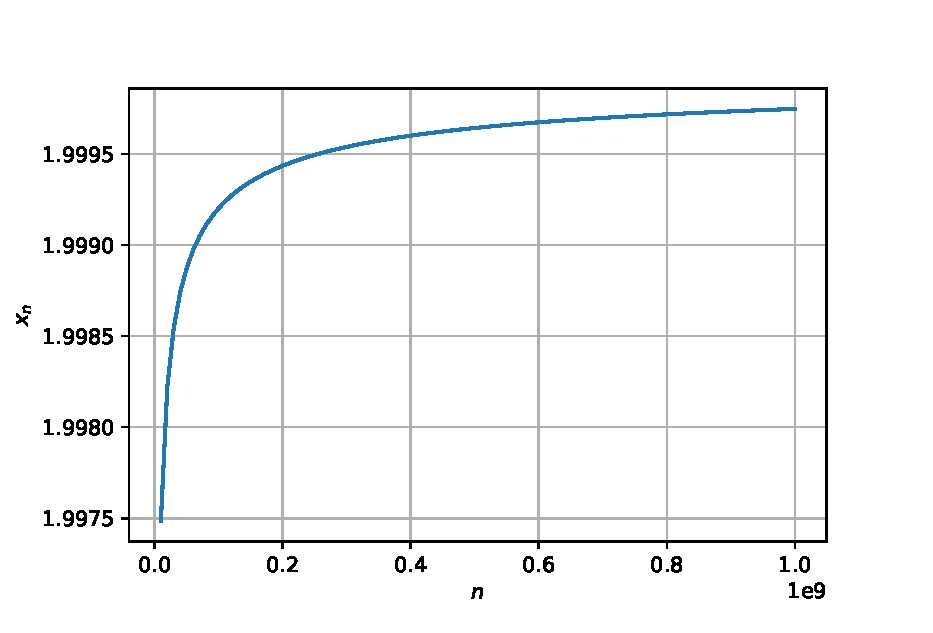
\includegraphics[width=\columnwidth]{./figs/seq_converge.eps}
\end{center}
\captionof{figure}{}
\label{fig:seq_converge}	
\end{figure}
%
\begin{definition}
\label{def:seq_converge}
The sequence $x_n$ converges to a limit $L$ if for $\epsilon > 0$, there exists an integer $K\brak{\epsilon} $ such that for all $n > K\brak{\epsilon}$,
%
\begin{align}
\abs{x_n - L} < \epsilon
\end{align}
%
\end{definition}
\begin{proposition}
\label{prop:archimedes}
Archimedian Property: For any real number $x$, there exists an integer $n > x$.
\end{proposition}
\begin{problem}
Guess the value of $L$ for $x_n$ in \eqref{eq:seq_converge} as $n \rightarrow \infty$.
\end{problem}
\solution From Fig. \ref{fig:seq_converge}, $L=2$.
\begin{problem}
Show that $x_n$ in \eqref{eq:seq_converge} converges to $L=2$ using Definition \ref{def:seq_converge}.
\end{problem}
\solution
\begin{align}
\abs{x_n - 2} &= \abs{\frac{2n}{n+4\sqrt{n}} - 2}
\\
&= \frac{8\sqrt{n}}{n+4\sqrt{n}} \\
&< \frac{8\sqrt{n}}{n} = \frac{8}{\sqrt{n}}
\end{align}
Using Proposition \ref{prop:archimedes}, choose $K\brak{\epsilon} >  \frac{64}{\epsilon^2}$ to be an integer. 
\begin{equation}
n > K\brak{\epsilon} \Rightarrow n > \frac{64}{\epsilon^2} \Rightarrow \frac{8}{\sqrt{n}} < \epsilon
\end{equation}
%
Thus, there exists $K\brak{\epsilon}$ such that $\abs{x_n -2} < \epsilon$.
\begin{problem}
Let $x_n = \frac{1}{\ln \brak{n+1}}$.
\begin{enumerate}
\item Find the value to which  $x_n$ converges.
\item Find $K\brak{\epsilon}$ when $\epsilon = \frac{1}{2}$ and $\epsilon = \frac{1}{10}$.
\end{enumerate}
\end{problem}
\section{Monotonicity and Boundedness}
\begin{definition}
A sequence $x_n$ is said to be monotonically {\em increasing} if
\begin{equation}
x_{n+1} > x_n
\end{equation}
$x_n$ is monotonically {\em decreasing} if $x_{n+1} < x_n$.
\end{definition}
\begin{definition}
The sequence $x_n$ is said to be bounded if for all $n > N $
%
\begin{equation}
\abs{x_n} < M
\end{equation}
%
for some positive real number $M$.
\end{definition}
\begin{problem}
\label{prob:monotone}
Consider the sequence defined by
\begin{equation}
\label{eq:monotone}
x_n = 
\begin{cases}
1 & n = 1
\\
\frac{x_{n-1}+1}{3} & n > 1
\end{cases}
\end{equation}
Is the sequence
\begin{enumerate}
\item Monotonic?
\item Bounded?
\end{enumerate}
\end{problem}
\solution The following code plots Fig. \ref{fig:seq_monotone}. It is obvious from the figure that $x_n$ is both monotonically decreasing as
well as bounded.
\lstinputlisting{./codes/seq_monotone.py}
\begin{figure}[!ht]
\begin{center}
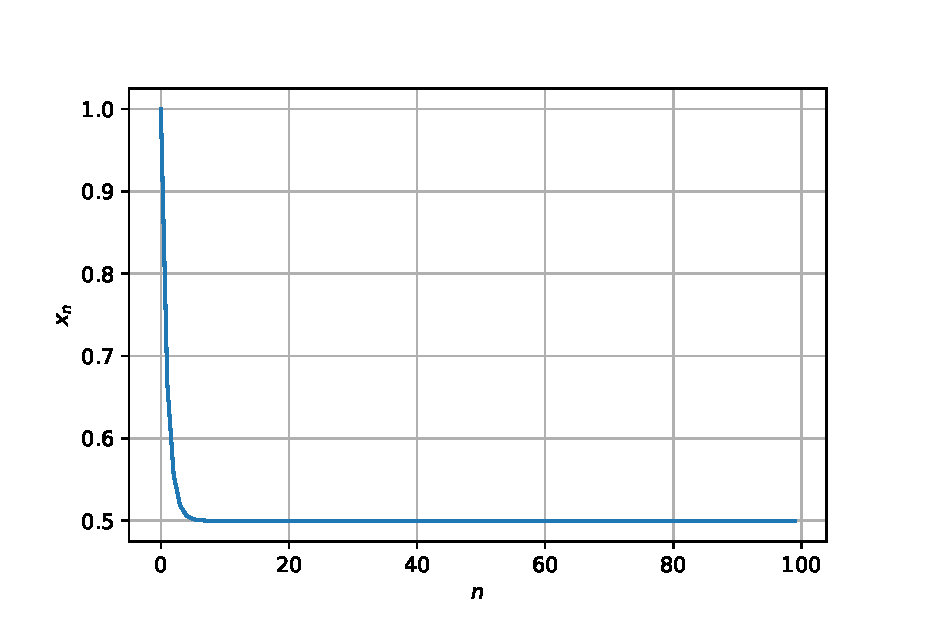
\includegraphics[width=\columnwidth]{./figs/seq_monotone.eps}
\end{center}
\captionof{figure}{}
\label{fig:seq_monotone}	
\end{figure}
\begin{problem}
Prove that $x_n$ is monotonically decreasing.
\end{problem}
\proof From \eqref{eq:monotone}, it can be shown that
\begin{align}
\label{eq:monotone_formula}
x_n  = \frac{1}{2}\brak{1 + \frac{1}{3^{n-1}}}
\end{align}
Thus,
\begin{align}
x_{n-1} - x_n = \frac{2}{3^{n-1}} > 0 \Rightarrow x_{n-1} > x_{n}
\end{align}
which is the condition for $x_n$ to be monotonically decreasing.
\begin{problem}
Prove that $x_n$ is monotonically decreasing using induction.
\end{problem}
\proof Since $x_1 = 1, x_2 = \frac{2}{3} < x_1$. Let $x_k < x_{k-1}$ . Then
%
\begin{align}
x_{k+1} - x_k &= \frac{x_k+1}{3}-\frac{x_{k-1}+1}{3}
\\
&= \frac{x_k - x_{k-1}}{3} < 0
\end{align}
%
Thus, $x_k < x_{k-1} \Rightarrow x_{k+1} < x_k$.  This shows that $x_n$ is decreasing.
\begin{problem}
Show that $x_n$ is bounded.
\end{problem}
\begin{proof}
From \eqref{eq:monotone_formula}, it is obvious that 
\begin{align}
\abs{x_n} \le 1
\end{align}
Thus, $x_n$ is bounded.
\end{proof}
\begin{problem}
Find the limit of $x_n$.
\end{problem}
\solution From Fig. \ref{fig:seq_monotone}, it is clear that the limit is $\frac{1}{2}$.
\begin{problem}
Show that the limit of $x_n$ is $\frac{1}{2}$.
\end{problem}
\begin{problem}
Show that the sequence defined by
%
\begin{equation}
x_n
=
\begin{cases}
2 & n = 1
\\
\sqrt{2x_{n-1}+1} & n > 1
\end{cases}
\end{equation}
%
is monotone as well as bounded.  Find its limit.
\end{problem}
\begin{proposition}
Any monotone sequence that is bounded is convergent.
\end{proposition}
\begin{problem}
\label{prob:seq_increasing}
Graphically show that $x_n = \sqrt{n+1} - 1$ is divergent.
\end{problem}
\solution The following code results in Fig. \ref{fig:seq_diverge}. It is obvious that the series does not converge.
\lstinputlisting{./codes/seq_diverge.py}
\begin{figure}[!ht]
\begin{center}
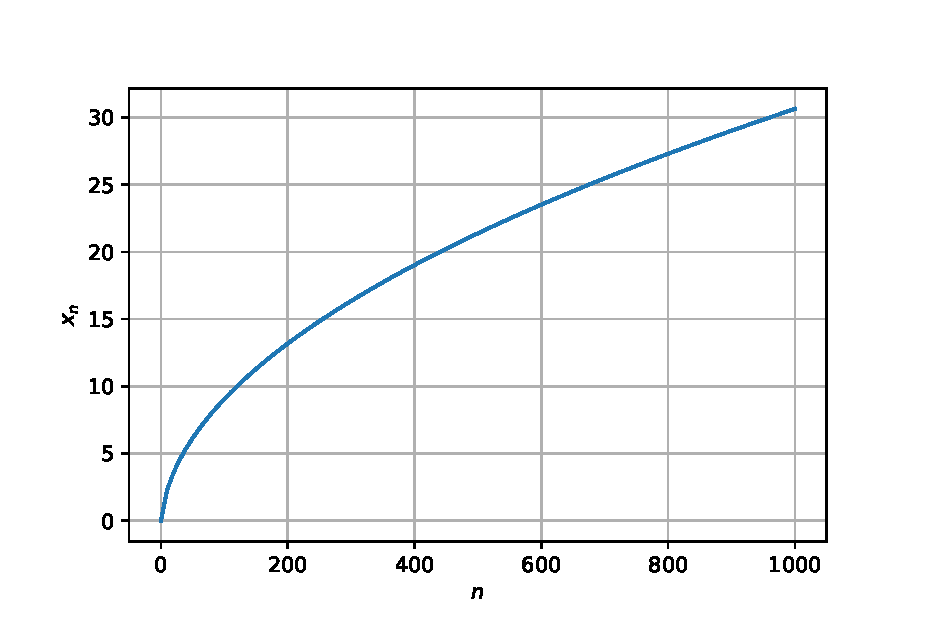
\includegraphics[width=\columnwidth]{./figs/seq_diverge.eps}
\end{center}
\captionof{figure}{}
\label{fig:seq_diverge}	
\end{figure}
\begin{problem}
Show that $x_n$ in Problem \ref{prob:seq_increasing} is increasing.
\end{problem}
\begin{proof}
Since $x_n > x_{n-1}$ for all $n$, the sequence is increasing.
\end{proof}
\begin{problem}
Show that $x_n$ in Problem \ref{prob:seq_increasing} is unbounded.
\end{problem}
\begin{proof}
For every $M$, it is possible to find an integer $n > M^2 - 1 \Rightarrow \sqrt{n+1} > M$.  Thus, $x_n$ is unbounded.
\end{proof}
\begin{proposition}
A monotone unbounded sequence is divergent.
\end{proposition}
\section{Cauchy Sequence}
\begin{definition}
The sequence $x_n$ is Cauchy if for every $\epsilon > 0$, there exists an integer $N$ such that
\begin{equation}
\abs{x_m-x_n} < \epsilon \quad \text{whenever } n,m \geq N 
\end{equation}
\end{definition}
\begin{problem}
Show that 
\begin{equation}
x_n = \frac{1}{n^2}
\end{equation}
is a Cauchy sequence.
\end{problem}
\proof Let $m > n > N$.
\begin{align}
\label{eq:cauchy_dist}
\abs{x_m-x_n} &= \abs{\frac{1}{m^2}-\frac{1}{n^2}} = \abs{\frac{\brak{m-n}\brak{m+n}}{m^2n^2}}
\end{align}
%Since $m > n$.  Thus, the denominator in \eqref{eq:cauchy_dist} 
%\begin{equation}
%m^2n^2 > n^4
%\end{equation}
The numerator in \eqref{eq:cauchy_dist}
\begin{equation}
\abs{\brak{m-n}\brak{m+n}} < 2m^2
\end{equation}
Thus, 
\begin{equation}
\abs{x_m-x_n} < \frac{2}{n^2} < \frac{2}{N^2} < \epsilon
\end{equation}
Thus it is possible to find an $N$ given $\epsilon$ for $x_n$ such that $x_n$ is Cauchy.
\begin{proposition}
Every Cauchy sequence is convergent and vice versa.
\end{proposition}
%
\begin{problem}
Show that
\begin{equation}
x_n = 1 + \frac{1}{2!}+ \frac{1}{3!}\dots + \frac{1}{n!}
\end{equation}
is a Cauchy sequence.
\end{problem}
\begin{problem}
Is $x_n = \sqrt{n}$ a Cauchy sequence?
\end{problem}

\end{document}

